\begin{figure}[ht]
  \caption[Compare the efficiency with tables saved as CSV and as parquet files]{This plot shows the runtime of the proposed method and the naive algorithm as they search for unique columns in tables of different sizes. I additionally compare the runtime reading the data from CSV files and reading it from parquet files.} % TODO: write better
  \label{fig:efficiency-shorter_loading_time-plot} % chktex 24
  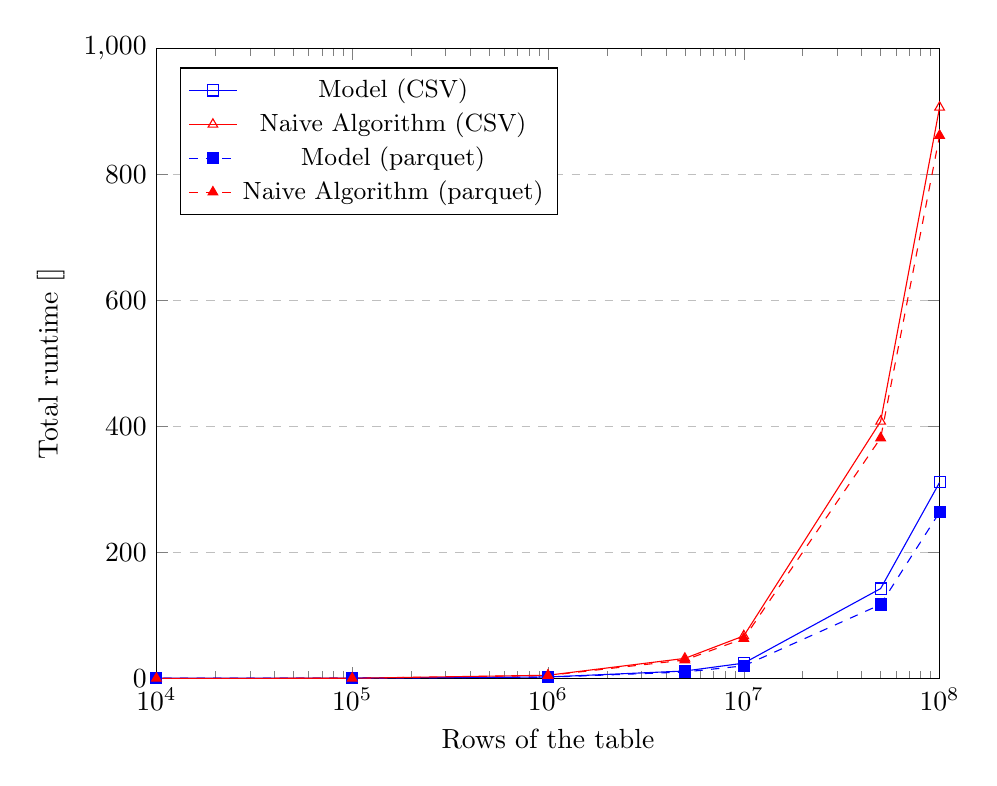
\begin{tikzpicture}
    \begin{axis}[
        % title={},
        xlabel={Rows of the table},
        ylabel={Total runtime [\si{\second}]},
        xmin=10000, xmax=100000000, xmode=log,
        ymin=0, ymax=1000,
        % xtick={0,1000,100000,10000000,100000000},
        % ytick={0,20,40,60,80,100,120},
        legend pos=north west,
        ymajorgrids=true,
        grid style=dashed,
        scale only axis,
        width={\linewidth-62pt},
        height=8cm
      ]

      % csv
      \addplot[
        color=blue,
        mark=square,
      ]
      coordinates {
          (100.0,1.0835406184196472) (1000.0,0.4514627978205681) (10000.0,0.4591604061424732) (100000.0,0.5741918832063675) (1000000.0,2.2600879333913326) (5000000.0,11.771335251629353) (10000000.0,24.25790297240019) (50000000.0,142.64984269440174) (100000000.0,311.1732710637152)
        };

      \addplot[
        color=red,
        mark=triangle,
      ]
      coordinates{
          (100.0,0.0039823874831199) (1000.0,0.0037141181528568) (10000.0,0.0264939442276954) (100000.0,0.3022922314703464) (1000000.0,5.0495885498821735) (5000000.0,31.796920645982027) (10000000.0,67.54112743958831) (50000000.0,408.1332451477647) (100000000.0,906.6464131213723)
        };

      % parquet
      \addplot[
        color=blue,
        mark=square*,
        dashed,
        mark options={solid}
      ]
      coordinates {
          (100.0,0.4577647559344768) (1000.0,0.4482727721333504) (10000.0,0.4571339413523674) (100000.0,0.5343325138092041) (1000000.0,1.90179156512022) (5000000.0,10.232811015099289) (10000000.0,19.938058882951736) (50000000.0,117.29449190944432) (100000000.0,263.89783180877566)
        };

      \addplot[
        color=red,
        mark=triangle*,
        dashed,
        mark options={solid}
      ]
      coordinates{
          (100.0,0.0062335357069969) (1000.0,0.0053194314241409) (10000.0,0.0245211236178874) (100000.0,0.2559473849833011) (1000000.0,4.6651470102369785) (5000000.0,29.216464921832085) (10000000.0,63.27469082176685) (50000000.0,381.673400811851) (100000000.0,861.8326124921441)
        };

      %       % parquet small_table
      %       \addplot[
      %         color=blue,
      %         mark=square,
      %       ]
      %       coordinates {
      % (100.0,0.4629099182784557) (1000.0,0.4608258455991745) (10000.0,0.4631855227053165) (100000.0,1.5644594952464104) (1000000.0,1.8686350099742413) (5000000.0,9.371084868907928) (10000000.0,19.90878576785326) (50000000.0,117.83388417959212) (100000000.0,261.4674338325858) 
      % };

      %       \addplot[
      %         color=red,
      %         mark=triangle,
      %       ]
      %       coordinates{
      % (100.0,0.0039786621928215) (1000.0,0.0044715628027915) (10000.0,0.024229060858488) (100000.0,0.2556539326906204) (1000000.0,4.715674605220556) (5000000.0,29.195809934288263) (10000000.0,63.66628506034613) (50000000.0,381.9564390294254) (100000000.0,861.1740412451327) 
      % };

      \legend{\small Model (CSV), \small Naive Algorithm (CSV), \small Model (parquet), \small Naive Algorithm (parquet)}

    \end{axis}
  \end{tikzpicture}
\end{figure}
